\chapter{Linux}\label{ch:linux}

Als ICT-er, en zeker als AI-specialist, zul je te maken krijgen met verschillende computersystemen en hiermee moeten kunnen werken. Voor cloud-servers specifiek is het waarschijnlijk dat je te maken krijgt met een niet-grafische Linux-omgeving. In dit hoofdstuk wordt gekeken naar Bash, de standaard login-shell voor Linux.

\section{Historie}\label{historie}

Linux is een afstammeling van de Unix traditie van besturingssystemen, die teruggaat tot Multics dat in de jaren 60 als time sharing OS voor de Multics GE-645 werd ontwikkeld door MIT, AT\&T Bell Labs en General Electric. Zoals te zien waren computers toen nog grote gedrochten, en was van de personal computer nog geen sprake. Een mainframe, zoals dit type computer heette, werd door hele bedrijven of afdelingen gedeeld. Programmeurs schreven code, waarna ze moesten wachten op hun beurt om de code te draaien. Als er een fout in zat, kon de programmeur opnieuw beginnen en een nieuwe beurt afwachten. Later werd het langzaam mogelijk met meerdere terminals (werkstations) de computer tegelijk te gebruiken. In deze context werd de grondslag voor Unix gelegd.

  \begin{marginfigure}
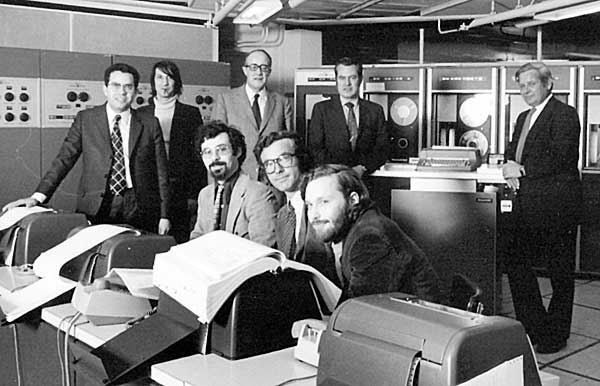
\includegraphics[width=0.8\textwidth]{ge645.jpg}\\
    GE-645 Mainframe {\scriptsize\emph (Image by Wikipedia)}\\[3mm]
  \end{marginfigure}

De ontwikkeling van Multics schoot niet op, waardoor Bell Labs besloot haar onderzoekers terug te trekken. Een deel daarvan, met name Ken Thompson, Dennis Ritchie en Brian Kernighan, ging bij Bell Labs verder met hun werk, maar op een kleinere schaal. Het resultaat hiervan is Unix. Unix had een eigen filosofie, waarbij alles als een file gezien werd (ook, bijvoorbeeld, devices). Hierdoor werd het makkelijker programma's aan elkaar te koppelen, met ``bestanden'' als koppelstukken. Dit leidde tot een filosofie van kleine, algemene programma's die oneindig in te zetten en te combineren waren. Dennis Ritchie vatte de filosofie samen als \emph{``What we wanted to preserve was not just a good environment in which to do programming, but a system around which a fellowship could form. We knew from experience that the essence of communal computing, as supplied by remote-access, time-shared machines, is not just to type programs into a terminal instead of a keypunch, but to encourage close communication.''}

  \begin{marginfigure}
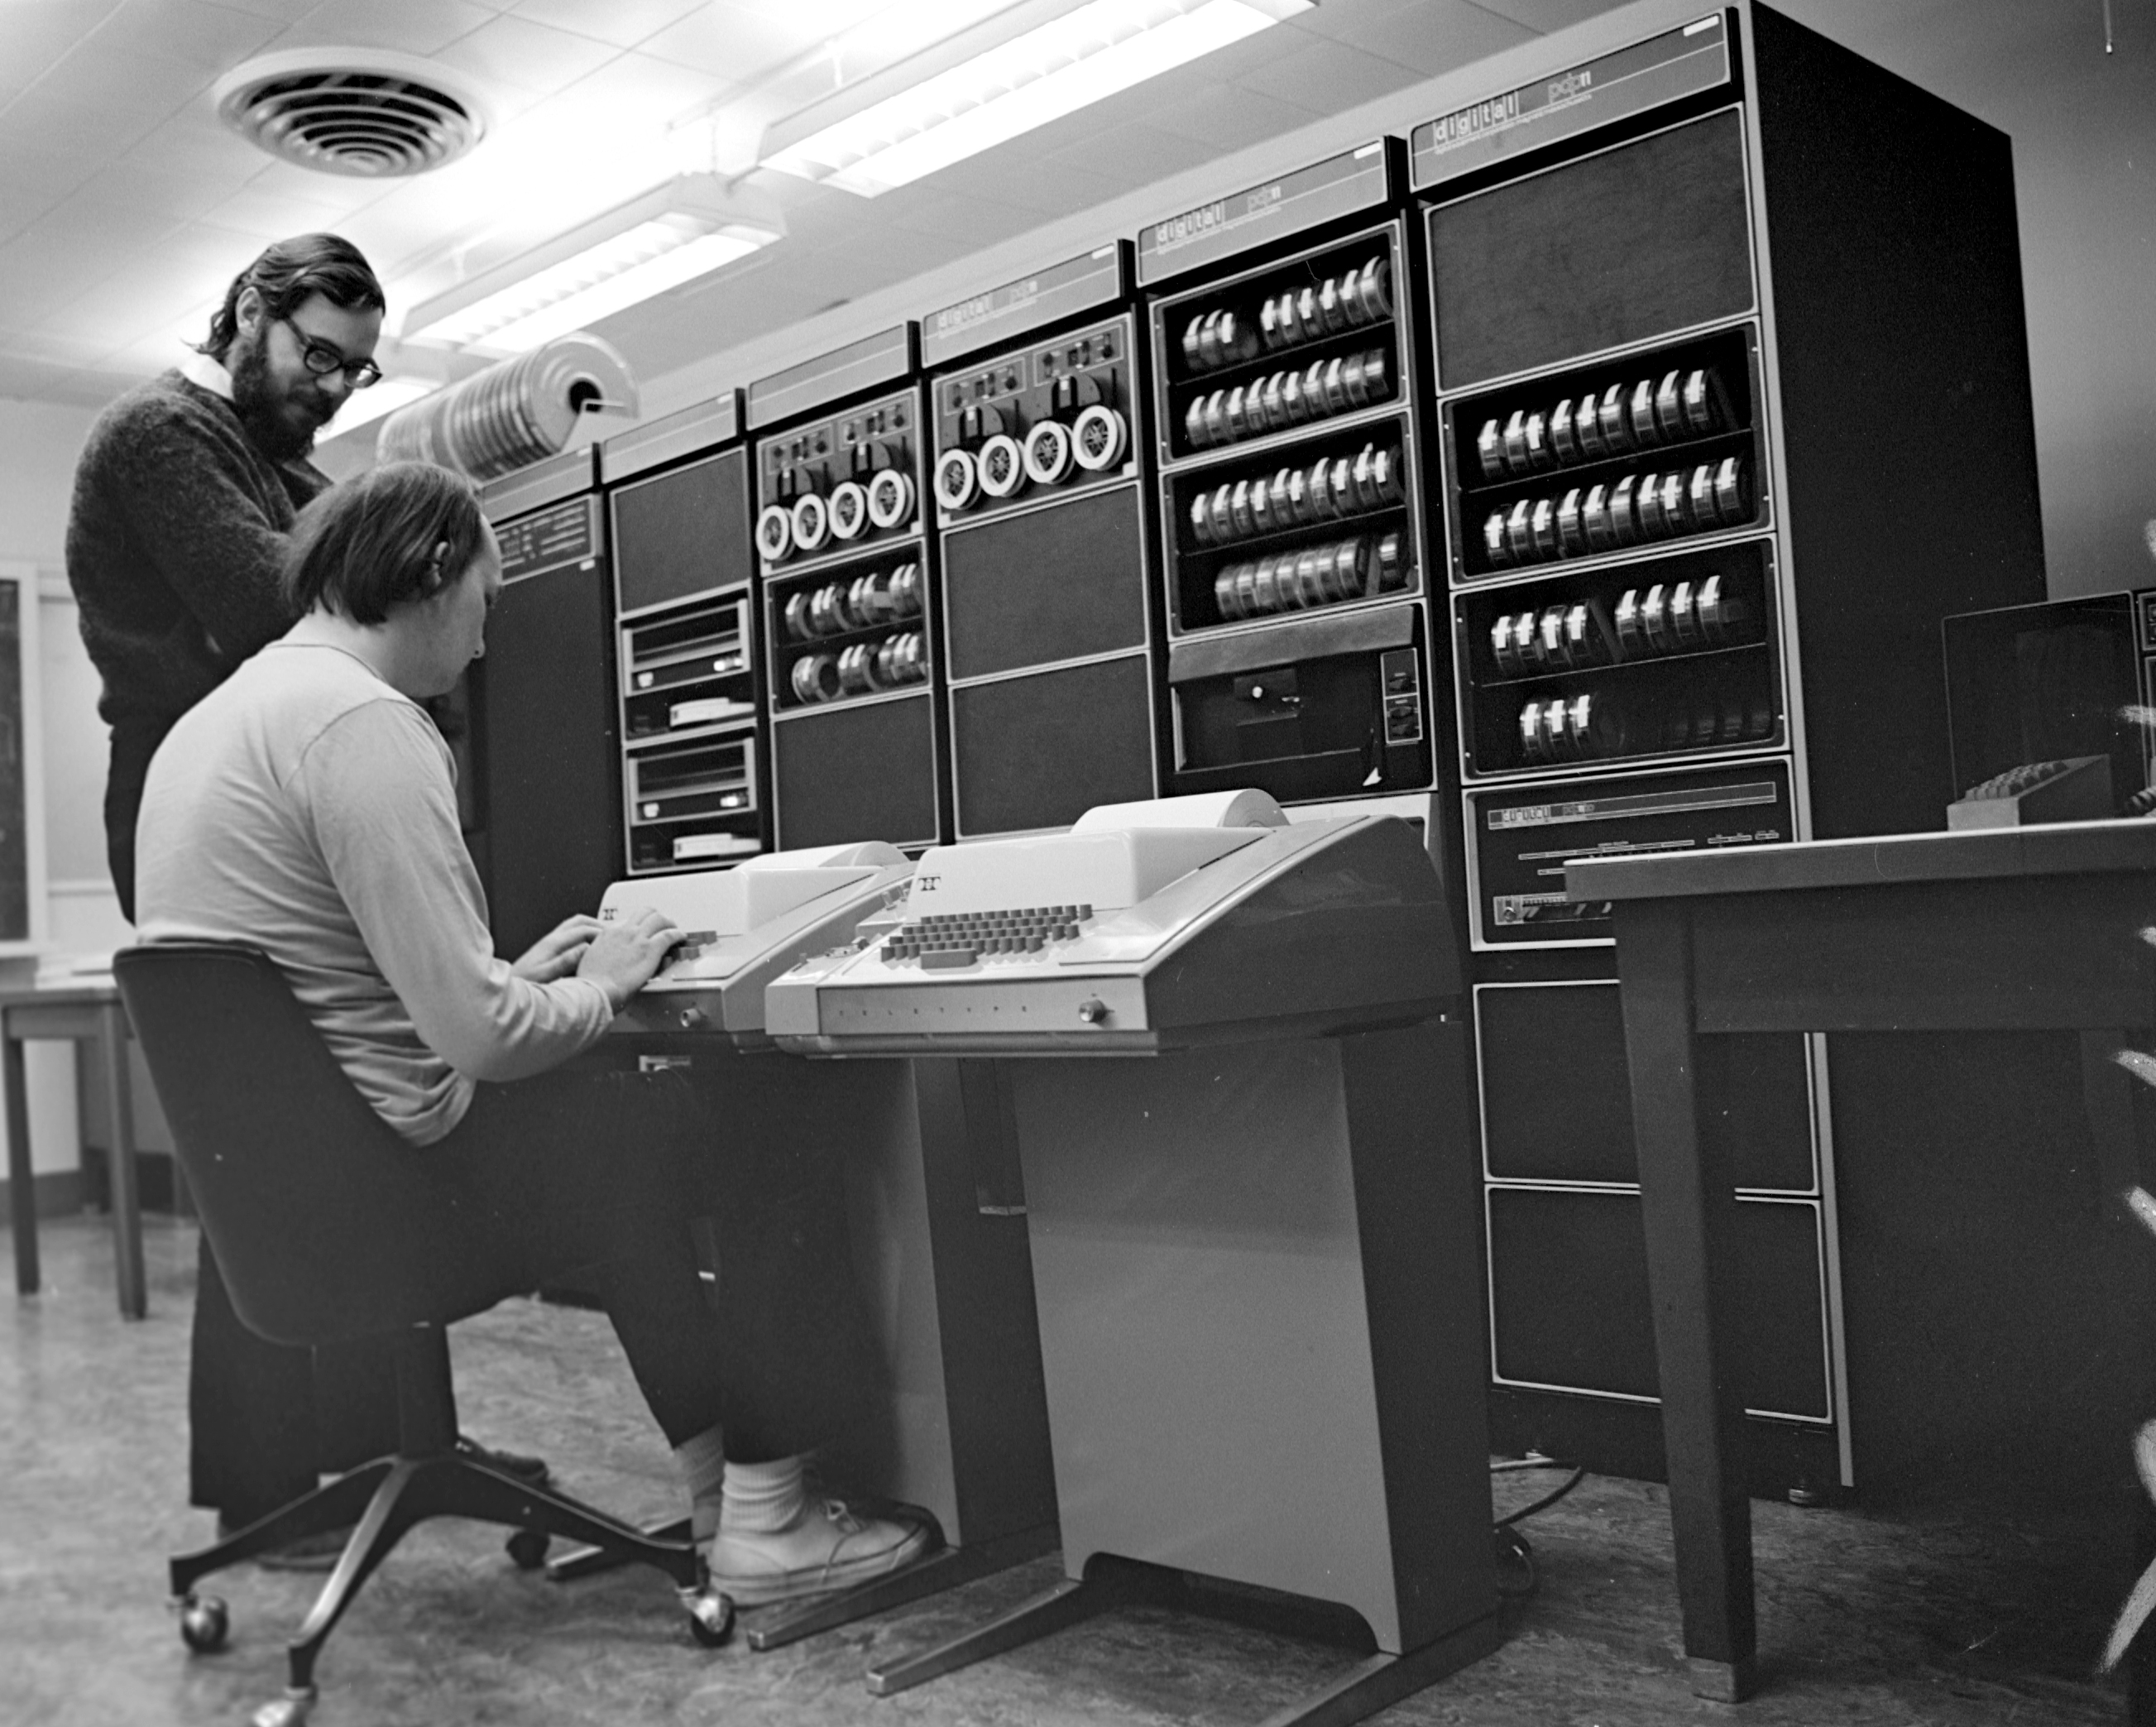
\includegraphics[width=0.8\textwidth]{thompson_ritchie.jpg}\\
    Thompson en Ritchie {\scriptsize\emph (Image by Wikipedia)}\\[3mm]
  \end{marginfigure}

De volgende stap richting Linux was Minix, geschreven door Andrew S. Tanenbaum. Minix was een erg versimpelde Unix afgeleidde die vooral educatief bedoeld was. De hele source-code, gecombineerd met de theorie waarop deze gebaseerd was, was als boek te koop (in het Turing Lab ligt een exemplaar). Hoewel de source-code beschikbaar was, was het niet toegestaan deze te verbeteren of te verspreiden. Daarnaast was de code vanuit educatief perspectief erg goed, maar praktisch gezien vooral al snel verouderd.

\subsection{Linux}\label{linux}

Linus Torvalds was een student informatica bij de Universiteit van Helsinki. Gebaseerd op het boek van Tanenbaum begon hij in 1991 met zijn eigen OS Kernel. Toen dit een beetje vorm begon te krijgen heeft hij dit \href{https://www.cs.cmu.edu/~awb/linux.history.html}{op usenet beschikbaar gesteld} voor wie er iets mee wilde.

  \begin{marginfigure}

\includegraphics[width=0.6\textwidth]{linus.jpg}\\
    Linus Torvalds {\scriptsize\emph (Image by Wikipedia)}\\[3mm]
  \end{marginfigure}

Ondertussen was Richard M. Stallman bezig met een eigen gratis (en vooral: open source) Unix vervanger: \href{https://www.gnu.org/}{GNU} (GNU's Not Unix). Dit was grotendeels compleet, alleen de kernel die hij ontwikkelde wilde geen kritieke massa krijgen. Omdat Linus bij zijn ontwikkeling gebruik had gemaakt van het werk dat voor GNU verzet was, was het een logische stap de twee projecten te combineren tot GNU/Linux. Hoewel we meestal gewoon Linux zeggen, is GNU/Linux de geprefereerde naam voor het hele OS.

  \begin{marginfigure}
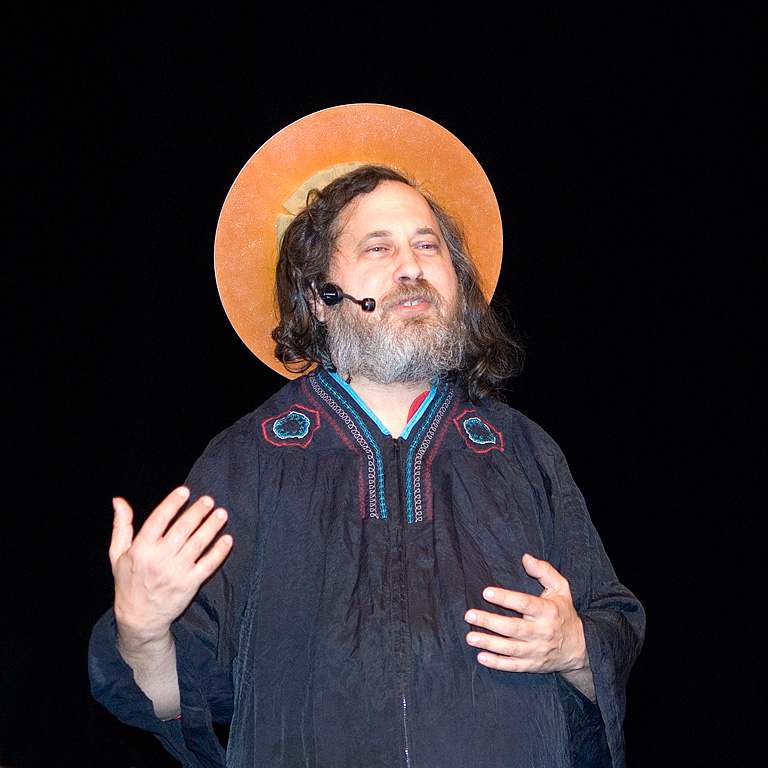
\includegraphics[width=0.6\textwidth]{rms.jpg}\\
    Richard Stallman {\scriptsize\emph (Image by Wikipedia)}\\[3mm]
  \end{marginfigure}

\subsection{Open Source}\label{open-source}

GNU en Linux vallen beide onder de \href{https://www.gnu.org/copyleft/gpl.html}{GNU General Public License}, een open source licentie. Dit houdt in dat de source code vrij beschikbaar is, mag worden aangepast en mag worden doorgegeven. Er is een grote diversiteit aan open source licenties in gebruik, en nog meer licenties die ruwweg dezelfde ideeën bevatten maar net niet aan de eisen voldoen om ``open source'' te mogen heten. Een deel van de open source licenties, waaronder de GPL, heeft een clausule die stelt dat hoewel je de code mag aanpassen, dat de resultaten daarvan ook onder dezelfde licentie moeten vallen. Andere open source licenties hebben deze eis niet. Merk op dat er geen verbod is op het verkopen van GPL software (of diensten daaromheen) of andere commerciële toepassingen (al zijn er licenties die dat wel hebben), zolang de source maar vrijelijk beschikbaar blijft. Later in deze les zullen we een aantal commerciële / betaalde toepassingen van Linux tegenkomen.

\section{De command-line}

In deze sectie maken we kennis met Bash, de meest gangbare shell voor Linux. Ook komen we een diversiteit aan programma's tegen die we vanaf de command line kunnen gebruiken. Het is in Bash niet altijd duidelijk welk commando een ``built-in'' functie van Bash is, en welk command een programma is: omdat Bash gebruikt wordt om programma's aan elkaar te knopen is deze grens behoorlijk vervaagd. Deze kennis is meestal ook niet nodig om Bash te gebruiken, maar wel iets om in het achterhoofd te houden.

\subsection{Je weg vinden op de command-line}\label{je-weg-vinden-op-de-command-line}

Als je een nieuwe terminal start\sidenote{of via bijvoorbeeld SSH een verbinding maakt}, heeft je shell standaard een working directory: het punt op het filesysteem waar je je bevindt. Bestanden die je maakt worden in deze map gezet, en bestanden die je zoekt kunnen relatief vanaf deze map benaderd worden. Standaard zul je beginnen in je \emph{home} directory, de map die je als gebruiker zelf beheert en waar je eigen bestanden (en instellingen) te vinden zijn. Het commando \texttt{cd} (change directory) wordt gebruikt om van map te wisselen, en \texttt{pwd} (present working directory) vertelt waar je je nu bevindt. Met \texttt{ls} (list) kun je de inhoud van de huidige map te zien krijgen. Een aantal paden zijn belangrijk om te weten: de bovenste directory, de root directory, wordt met een \texttt{/} (slash) aangeduid. Vanaf hier worden directory-namen door een \texttt{/} gescheiden om een pad uit te drukken. De home directory van de gebruiker \texttt{linus} bevindt zich bijvoorbeeld op \texttt{/home/linus} (de map \texttt{linus}, binnen de map \texttt{home}, binnen de root). \texttt{\textasciitilde} wordt gebruikt als synoniem voor de home directory van de huidige gebruiker. Voor linus is \texttt{cd\ \textasciitilde} dus hetzelfde als \texttt{cd\ /home/linus}. \texttt{.} verwijst naar de huidige map: \texttt{cd\ .} doet niets. Dit kan voor nu een beetje overbodig lijken, maar later zullen we zien hoe de \texttt{.} soms korter is dan de alternatieven. Daarnaast hebben we \texttt{..}, die naar de parent van de huidige directory verwijst. Vanaf Linus's home zal \texttt{cd\ ..} dus naar \texttt{/home} verwijzen. Deze kun je ook middenin een pad gebruiken, de map omhoog wordt dan gerekend vanaf waar in het pad deze wordt gebruikt. \texttt{cd\ /home/linus/Documents/../Music} is bijvoorbeeld hetzelfde als \texttt{cd\ /home/linus/Music}. \texttt{cd} zonder argument gaat terug naar de home directory, en \texttt{cd\ -} gaat terug naar de vorige directory.

\begin{bash}
\p cd Documents\\
\  \\
\p[\textasciitilde/Documents] pwd\\
/home/linus/Documents\\\\
\  \\
\p[\textasciitilde/Documents] cd ..\\
\  \\
\p cd Folder\\
\  \\
\p[\textasciitilde/Folder] cd ..\\
AnotherFile  File\\
\  \\
\p[\textasciitilde/Folder] cd \asciitilde\\
\  \\
\p cd -\\
/home/linus/Folder
\  \\
\p[\textasciitilde/Folder] cd .\\
\  \\
\p[\textasciitilde/Folder] cd /\\
\  \\
\p[/] ls\\
bin/  boot/  dev/  etc/  home/  media/  mnt/  proc/  root/  run/  sys/  tmp/  usr/  var/\\
\  \\
\p[/] cd\\
\  \\
\p pwd\\
/home/linus\\
\end{bash}

De volgende commando's manipuleren bestanden. Met \texttt{touch} wordt een bestand aangemaakt (als deze nog niet bestond) of wordt de ``laatst aangepast'' datum naar nu gezet. Het bestand wordt gewijzigd, maar er verandert niets aan. Met \texttt{cp} kun je een bestand kopiëren, en met \texttt{mv} kun je het verplaatsen. \texttt{rm} verwijdert een bestand.

\begin{bash}
\p ls\\
AnotherFile  File\\
\\
\p touch File3\\
\\
\p ls\\
AnotherFile  File  File3\\
\\
\p cp File File2\\
\\
\p ls\\
AnotherFile  File  File2  File3\\
\\
\p mv AnotherFile File1\\
\\
\p ls\\
File  File1  File2  File3\\
\\
\p rm File3\\
\\
\p ls\\
File  File1  File2\\
\end{bash}

De meeste commando's voor bestanden werken niet direct op directories. \texttt{mv} mag, maar \texttt{cp} en \texttt{rm} werken niet. Voor het verwijderen van een \emph{lege} map wordt \texttt{rmdir} gebruikt, maar dit mag niet als er een bestand in de map zit. Dit is omdat Linux je wil beschermen geen verkeerde handeling uit te voeren: als je aangeeft dat je een bestand wil verwijderen, maar je geeft een map op, dan is de kans groot dat je de verkeerde naam hebt meegegeven. Als je toch een map (met alle inhoud) wilt kopiëren of verwijderen, kun je \texttt{cp\ -r} en \texttt{rm\ -r} gebruiken. De toevoeging \texttt{-r} staat voor \emph{recursief} (dat betekent in dit geval: met alles wat eronder hangt). Gebruik bijvoorbeeld \texttt{rm\ -r\ Music} als je de map Music met alle inhoud wil verwijderen. \texttt{-r} is het eerste voorbeeld van een flag.

\begin{bash}
\p[~/Folder] ls\\
File  File1  File2\\
\\
\p[~/Folder] mkdir Subfolder\\
\\
\p[~/Folder] touch Subfolder/File\\
\\
\p[~/Folder] mkdir EmptyFolder\\
\\
\p[~/Folder] ls\\
EmptyFolder/  File  File1  File2  Subfolder/\\
\\
\p[~/Folder] mkdir EmptyFolder2\\
\\
\p[~/Folder] ls\\
EmptyFolder/  EmptyFolder2/  File  File1  File2  Subfolder/\\
\\
\p[~/Folder] rmdir EmptyFolder\\
\\
\p[~/Folder] rmdir Subfolder\\
rmdir: failed to remove 'Subfolder/': Directory not empty\\
\\
\p[~/Folder] cp Subfolder Backup\\
cp: -r not specified; omitting directory 'Subfolder'\\
\\
\p[~/Folder] cp -r Subfolder Backup\\
\\
\p[~/Folder] ls\\
Backup/  EmptyFolder2/  File  File1  File2  Subfolder/\\
\\
\p[~/Folder] rm -r Subfolder\\
\\
\p[~/Folder] rm -r EmptyFolder2\\
\\
\p[~/Folder] ls\\
Backup/  File  File1  File2\\
\end{bash}

\subsection{Flags / Command Line Arguments}\label{flags-command-line-arguments}

De meeste commando's accepteren command line argumenten. Allereerst zijn er verplichte argumenten. Waar \texttt{pwd} bijvoorbeeld geen argumenten nodig heeft, heeft \texttt{touch} enkel zin als meegegeven wordt welk bestand gemaakt of geüpdatet moet worden. \texttt{cp} heeft zelfs twee argumenten nodig: een bron en een doel. Soms kan een commando een optioneel pad meekrijgen: \texttt{ls} werkt in de huidige working directory, \texttt{ls\ /home} leest de inhoud van \texttt{/home}. Al deze argumenten zijn positie-bepaald. Het eerste argument bij \texttt{cp} is altijd de bron, de tweede het doel. Naast deze positiegebonden argumenten hebben we ook flags, die met één of twee streepjes (dashes) kunnen beginnen. Flags komen doorgaans overeen met booleaanse waardes: wel of niet. Als de flag met één dash begint, dan is het doorgaans een enkele letter, en kun je deze combineren. \texttt{-r\ -f} is hetzelfde als \texttt{-rf}; het maakt niet uit of je \texttt{rm\ -r\ -f\ Music} gebruikt of het kortere \texttt{rm\ -rf\ Music}. Ook de volgorde maakt meestal niet uit. Flags met een dubbele dash bestaan uit meerdere letters en zijn niet samen te voegen. Tot slot kunnen deze flags soms een argument erbij nemen. Bij enkele letters volgt het argument meestal na een (optionele) spatie, bij de dubbele dash wordt meestal een \texttt{=} gebruikt om de waarde van de flag te scheiden.

\begin{bash}
\p[~/Folder] ls\\
File  File1  File2  Folder1/  Folder2/ Folder3/\\
\\
\p[~/Folder] rm -r Folder1    \# Recursive om directory te deleten\\
\\
\p[~/Folder] rm -f File2      \# Force remove\\
\\
\p[~/Folder] rm -r -f Folder2 \# Force recursive remove\\
\\
\p[~/Folder] rm -rf Folder3   \# Zelfde als -r -f\\
\\
\p[~/Folder] rm --force File1 \# Zelfde als -f\\
\\
\p[~/Folder] ls\\
File\\
\end{bash}

Sommige commando's hebben erg veel opties om de gewenste functionaliteit te selecteren. De meeste commando's hebben een \texttt{-h} en/of \texttt{-\/-help} optie om wat tips te geven over het gebruik. Voor het hele verhaal kun je \texttt{man} gebruiken, oftewel de manual.

\begin{bash}
\p[~] rm --help\\
\# Print een (relatief) korte handleiding\\
\\
\p[~] man rm\\
\# Scroll door de uitgebreide handleiding\\
\end{bash}

\subsection{IO en Pipes}\label{io-en-pipes}

Om een tree te krijgen van de inhoud van een map en alle submappen kun je het commando \texttt{find} gebruiken. Dit geeft echter vrij veel uitvoer, het zou fijn zijn als we hier hapklare brokken van konden maken. Het commando \texttt{less} kan gebruikt worden om een bestand te openen en er doorheen te kunnen scrollen. Kunnen we dit gebruiken om de uitvoer van \texttt{find} te pagineren? In Linux kun je twee commando's aan elkaar koppelen: uitvoer van het ene programma wordt als invoer voor het tweede gebruikt. Hiervoor gebruiken we het \texttt{\textbar{}} symbool: de pipe. Denk aan een pijpleiding die de commando's met elkaar verbindt.

\begin{bash}
\p[~] find /home/linus\\
\# Print de hele mappenstructuur; veel output\\
\\
\p[~] less file\\
\# Lees een bestand door er doorheen te scrollen\\
\\
\p[~] find /home/linus | less\\
\# Combineer de tools: scroll door de uitvoer van find\\
\end{bash}


\newthought{Pipes zijn een fundamenteel deel van de Unix filosofie} om eenvoudige programma's te combineren voor complex gedrag. Het sturen van de uitvoer noemen we het \emph{redirecten} van \texttt{STDOUT} (standard out), en het lezen van de invoer is het \emph{redirecten} van \texttt{STDIN} (standard in). Dit hoeft niet met een pipe te gebeuren, maar kan ook van/naar een bestand. \texttt{STDOUT} is een file descriptor (nummer 1) die in ieder proces aanwezig is, en die gebruikt wordt om alles naartoe te schrijven dat het programma uitvoert (denk aan \texttt{print}s). \texttt{STDIN} is ook een file descriptor (nummer 0), maar deze wordt gelezen voor invoer. Normaal is dit de gebruikersinvoer vanaf de command line, maar dit kan ook prima een bestand of pipe zijn. Daarnaast is er vaak een derde file descriptor, \texttt{STDERR} (standard error, nummer 2), voor foutmeldingen (ook dit is standaard de command line, maar het is hiermee dus mogelijk te splitsen tussen uitvoer en excepties). Het gebruik van file descriptors voor de invoer/uitvoer is weer een voorbeeld van de UNIX-filosofie dat alles een bestand is. Een descriptor is de datastructuur die UNIX intern gebruikt om iets te kunnen benaderen; een file descriptor verwijst dus naar een bestand (en hoe dit gelezen/geschreven kan worden). Waar \texttt{STDIN} en \texttt{STDOUT} precies aan verbonden zijn, is te vinden in de environment informatie die bij een proces hoort. Standaard zijn dit voor processen die je in de shell start de invoer en de uitvoer van de terminal, en als je een child process start worden deze overgeërfd. Tijdens executie van het proces kunnen deze descriptors altijd worden gesloten of ergens anders aan verbonden worden. Bij processen die door de kernel gestart worden, zoals \texttt{init} is de \texttt{STDOUT} doorgaans aan het kernel log gekoppeld. \texttt{STDIN} kan aan een buffer of (als het proces geen input verwacht) aan een dummy file gekoppeld zijn: een lege file descriptor die niet aan een daadwerkelijk bestand op de schijf gekoppeld is.

\begin{figure}[ht]
    \centering
    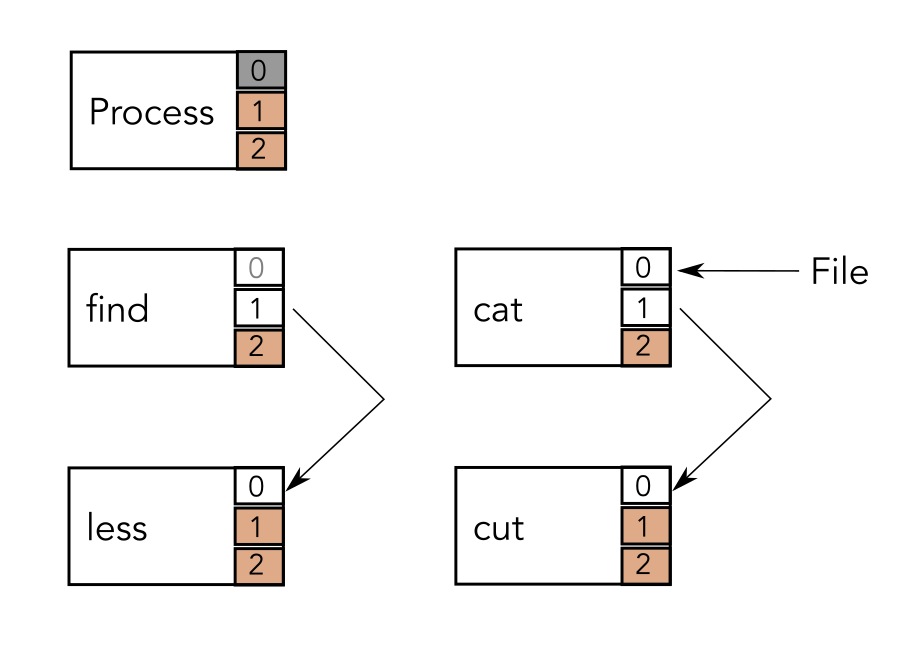
\includegraphics[width=\textwidth]{io.png}
    \caption{File Descriptors van een Proces}
    \label{fig:process-io}
\end{figure}

Net als dat we vanaf de shell twee commando's aan elkaar kunnen pipen, kunnen we ook een file descriptor meegeven om als \texttt{STDIN}, \texttt{STDOUT} of \texttt{STDERR} te gebruiken. Dit kan respectievelijk met \texttt{\textless{}}, \texttt{\textgreater{}} en \texttt{2\textgreater{}}. Je kunt bijvoorbeeld \texttt{find\ /home/linus\ \textgreater{}\ filetree} gebruiken om de uitvoer van \texttt{find\ /home/linus} in het bestand \texttt{filetree} te schrijven. Bij \texttt{find\ /home/linus\ 2\textgreater{}\ errors.log} wordt niet de uitvoer verbonden, maar eventuele foutmeldingen via \texttt{STDERR}. Als het bestand waarnaar je wilt uitvoeren al bestaat, wordt het als je \texttt{\textgreater{}} gebruikt overschreven, maar je kunt, \texttt{\textgreater{}\textgreater{}} en \texttt{2\textgreater{}\textgreater{}} gebruiken om in plaats daarvan achteraan het bestand toe te voegen. Tot slot kun je \texttt{\textless{}\textless{}\ MARKER} of \texttt{\textless{}\textless{}-\ MARKER} (een zogenaamde ``heredoc'') gebruiken om \texttt{STDIN} vanaf de command line mee te geven, tot aan de eerste regel met enkel \texttt{MARKER}. Dit maakt het makkelijk meerdere regels tekst mee te geven. De toegevoegde waarde van de \texttt{-} is dat deze een tab aan het begin van een regel negeert en mogelijk leesbaarder is. Op zichzelf wordt \texttt{\textless{}} niet zo veel gebruikt, omdat de meeste programma's standaard een meegegeven bestandsnaam als \texttt{STDIN} interpreteren (dus \texttt{less\ \textless{}\ file} is hetzelfde als \texttt{less\ file}), maar bij sommige programma's kan dit nodig zijn. Een voorbeeld is \texttt{psql}, een database waarbij je een bestand met instructies mee kan geven met \texttt{psql\ databasename\ \textless{}\ sqlfile}. Als je \texttt{\textless{}} niet gebruikt en vanaf de command line invoert kun je \texttt{Control-d} gebruiken om je invoer te beëindigen, in plaats van de explicete \texttt{MARKER} die je bij \texttt{\textless{}\textless{}} gebruikt. \texttt{wc} staat trouwens voor \emph{word count}, waarbij \texttt{wc\ -l} het aantal regels telt, en \texttt{wc\ -c} het aantal karakters.

\begin{bash}
\p[~] find /home/linus > filetree 2> errors.log\\
\# Geen output; alles staat in bestanden filetree en errorslog\\
\\
\p[~] wc -l filetree >\!> filetree\\
\# Het totaal aantal regels in filetree wordt onderaan filetree toegevoegd\\
\\
\p[~] wc -c <\!< EOF\\
> Lorem Ipsum\\
> Dolor Sit Amet\\
> EOF\\
27\\
\\
\p[~] psql databasename < sqlfile\\
\# Laadt een database uit een file\\
\end{bash}

\subsection{Meer Commando's met Pipes}\label{meer-commandos-met-pipes}

Nu we het bestaan van pipes kennen, zijn hier nog wat commando's die op zichzelf niet altijd even zinvol zijn, maar als deel van een pipeline goed werken. Om uit bestand (of uitvoer) regels te filteren die een bepaalde string bevatten kun je \texttt{grep} gebruiken. \texttt{sort} geeft de invoer gesorteerd terug, en \texttt{cut} snijdt per regel een substring uit. In het onderste voorbeeld wordt \texttt{ls\ -l} gebruikt (een directory listing met uitgebreide info). We gebruiken \texttt{cut\ -c14-} om karakter 14 tot eind te bewaren, waardoor de eigenaar van het bestand vooraan komt te staan. Met \texttt{sort} kunnen we hierop sorteren.

\begin{bash}
\p[~/Folder] ls -la\\
total 0\\
drwxr-xr-x 1 linus users   44 Jan 28 10:10 .\\
drwx------ 1 linus users 6142 Jan 28 10:05 ..\\
-rw-r--r-- 1 root  users    0 Jan 28 09:46 File\\
-rw-r--r-- 1 linus users    0 Jan 28 10:08 File2\\
-rw-r--r-- 1 linus users    0 Jan 28 10:08 File2025\\
-rw-r--r-- 1 linus users    0 Jan 28 10:08 File3\\
\\
\p[~/Folder] ls -la | grep 2025\\
-rw-r--r-- 1 linus users 0 Jan 28 10:08 File2025\\
\\
\p[~/Folder] ls -la | cut -c14- | sort\\
\\
linus users    0 Jan 28 10:08 File2\\
linus users    0 Jan 28 10:08 File2025\\
linus users    0 Jan 28 10:08 File3\\
linus users   44 Jan 28 10:10 .\\
linus users 6142 Jan 28 10:05 ..\\
root  users    0 Jan 28 09:46 File\\
\end{bash}

\subsection{Pipelines en Command-lists}\label{pipelines-en-command-lists}

Meerdere commands gescheiden door pipes vormen samen een pipeline. De commando's worden parallel uitgevoerd. Je kunt ook meerdere commands na elkaar uit laten voeren, dit kan met de puntkomma en wordt een command-list genoemd. Het is zelfs mogelijk meerdere pipelines in een command list te zetten.

\begin{bash}
\p[~] foo | bar\\
\# De uitvoer van foo gaat naar bar\\
\\
\p[~] foo ; bar\\
\# bar wordt na foo uitgevoerd\\
\\
\p[~] foo | bar ; baz | quux\\
\# Eerst worden foo en bar uitgevoerd, waarbij de uitvoer van foo naar bar gaat\\
\# Als dit klaar is worden baz en quux gestart, en gaat de uitvoer van baz naar quux\\
\end{bash}

Commands in een command list worden na elkaar uitgevoerd, ongeacht of er ergens iets mis gaat. Soms wil je het tweede command enkel uitvoeren als het eerste command geslaagd is, of juist alleen als er een fout is geweest. Zoals we weten heeft ieder command een exit status, \texttt{0} voor succes of iets anders voor een fout. Door \texttt{\&\&} tussen commands te zetten, in plaats van \texttt{;} wordt het tweede commando alleen uitgevoerd als het eerste geslaagd is. De dubbele pipe \texttt{\textbar{}\textbar{}} werkt precies andersom: het tweede command wordt alleen uitgevoerd als de eerste mislukte. We noemen deze operators \emph{en} en \emph{of}. ``Doe a en b'' kan alleen maar als \emph{a} gelukt is, zo niet zal de shell het meteen opgeven. ``Doe a of b'' levert de shell een alternatief, probeer eerst \emph{a}, en als dat niet lukt, doe dan \emph{b}.

\begin{bash}
\p[~] foo || bar\\
\# bar wordt uitgevoerd als foo faalt\\
\\
\p[~] foo && bar\\
\# bar wordt uitgevoerd als foo gelukt is\\
\end{bash}

\subsection{Procesmanagement}\label{procesmanagement}

Als je wilt weten welke processen er op dit moment actief zijn kun je het commando \texttt{ps} gebruiken. Normaal geeft dit alleen een lijst met je eigen processen in terminals, maar met \texttt{ps\ -A} krijg je alle processen te zien. De standaarduitvoer geeft (afhankelijk van je distributie) in ieder geval de PID, terminal en het command. Vaak wordt ook de effectieve tijd die het proces gedraaid heeft meegegeven (effectieve tijd telt alleen de tijd dat het proces daadwerkelijk actief was). Daarnaast heeft \texttt{ps} nog heel veel opties om processen te selecteren en aan te geven welke informatie je wel en niet wil hebben, zie daarvoor de \texttt{man} pagina. \texttt{ps} geeft een eenmalige uitvoer van de processenlijst op dat moment; dit is handig als je dit met andere commands in een pipeline wil combineren. Soms wil je echter een dynamische lijst die zichzelf update, zoals het taakbeheer in Windows. Hier is het commando \texttt{top} voor, of de verbeterde versie \texttt{htop} (meestal niet standaard geïnstalleerd). Tot slot kan je een proces vanaf de command line beëindigen (op voorwaarde dat je zelf de eigenaar van het proces bent). Hiervoor gebruik je \texttt{kill} met de PID van het proces, of \texttt{killall} met de naam van het proces. De laatste heet killall, omdat het goed kan zijn dat je meerdere instanties van dezelfde executable open hebt staan. \texttt{killall\ firefox} sluit bijvoorbeeld alle Firefox vensters, niet een specifieke.

\begin{bash}
\p[~] ps\\
\# geef de processen binnen de huidige shell\\
\\
\p[~] ps -A\\
\# geef alle processen\\
\\
\p[~] top\\
\# interactieve "task manager"\\
\\
\p[~] kill\\
\# stop een proces met een gegeven PID\\
\\
\p[~] killall\\
\# stop elk proces met een gegeven naam\\
\end{bash}

\subsection{Signals}\label{signals}

\texttt{kill} en \texttt{killall} zullen standaard een \texttt{SIGTERM} signaal naar een proces sturen: een vriendelijk doch dringend verzoek om op te houden te bestaan. Dit betekent dat het proces de gelegenheid heeft achter zich op te ruimen, de gebruiker te vragen of zij de wijzigingen op wil slaan, of het verzoek te negeren. Er bestaan echter meerdere signalen die je kan sturen, de belangrijksten staan in de tabel hieronder. Om bijvoorbeeld een \texttt{SIGKILL} signaal te versturen (om een proces direct en \emph{with extreme prejudice} om zeep te helpen) kan dit met \texttt{kill\ -SIGKILL}. \texttt{SIGSTOP} pauzeert een proces, dat met \texttt{SIGCONT} weer hervat kan worden. In de tussentijd is het proces bevroren, en zal het niet gescheduled worden. Een GUI applicatie zal wel een scherm behouden, maar nergens meer op reageren tot het een \texttt{SIGCONT} ontvangt. De tabel met beschikbare signalen is groot, en bevat ook signalen die normaal alleen voor intern gebruik zijn: \texttt{SIGSEGV} wordt bijvoorbeeld door de kernel gestuurd als een proces buiten zijn geheugenruimte opereert (een Segmentation Fault), en \texttt{SIGFPE} wordt onder andere door de CPU gestuurd naar een proces dat door 0 probeert te delen. De hele tabel is in de Linux documentatie of op internet te vinden. De getallen zijn de interne waardes die het OS herkent, de namen zijn enkel om het de gebruiker makkelijker te maken.

\begin{itemize}
  \item \texttt{SIGKILL(9)} Proces beëindigen, kan niet afgevangen worden \\
  \item \texttt{SIGUSR1(10)} User defined, verschilt per programma \\
  \item \texttt{SIGTERM(15)} Standaard signaal, ``sterf, alsjeblieft'' \\
  \item \texttt{SIGCONT(18)} Hervat een gestopt (gepauseerd) proces \\
  \item \texttt{SIGSTOP(19)} Stop tot je een SIGCONT krijgt \\
\end{itemize}

\subsection{Fore- en Background jobs}\label{fore--en-background-jobs}

Doorgaans zal een shell bij het uitvoeren van een command een \texttt{fork()} en een \texttt{exec()} uitvoeren, waarna de parent \texttt{wait()} tot het kind klaar is. Met behulp van de enkele ampersand (\texttt{\&}) kunnen we een proces op de achtergrond starten: de shell wacht niet en geeft meteen een nieuw prompt aan de gebruiker. Het nieuwe proces is nog steeds een kind van de shell, en als de shell beëindigd wordt voor het kind klaar is wordt dit ook getermineerd. Met \texttt{Control-z} kun je het huidige foreground proces (het proces waarop de shell aan het wachten is) een \texttt{SIGSTOP} sturen, waarna de shell weer op de gebruiker kan reageren. Met \texttt{fg} krijgt het proces een \texttt{SIGCONT} en hervat het de claim op de shell: het wordt naar de voorgrond gestuurd. Je kunt echter ook \texttt{bg} gebruiken om het proces op de achtergrond door te laten gaan, net alsof het met een \texttt{\&} gestart was. \texttt{jobs} geeft een lijst met actieve achtergrond processen. Als je een shell met actieve achtergrondprocessen probeert te beëindigen krijg je meestal een waarschuwing: als de terminal sluit stoppen de processen ook. Om dit te voorkomen kun je het proces met \texttt{disown} onterven: het is niet langer een kind van de shell waar het gestart is, maar wordt onder het \emph{init} proces gehangen.

\begin{bash}
\p[~] python3\\
Python 3.13.0b4 (main, Jul 18 2024, 09:41:38) [GCC 13.3.0] on linux \\
Type "help", "copyright", "credits"\  or "license"\ for more information.\\
>\!>\!> antwoord = 42\\
>\!>\!> \\
[1]+  Stopped                 python3                  \# Python gepauzeerd ("Stopped")\\
\\
\p[~] ls Folder                                \# Terug in Bash\\
File File2 File2025 File3\\
\\
\p[~] jobs\\
[1]+  Stopped                 python3\\
\\
\p[~] fg                                       \# Terug in Python, waar we gebleven waren\\
python3                                                \# Bash vertelt nog welk proces er draait\\
print(antwoord)                                        \# Geen >\!>\!> (die staat hierboven al)\\
42\\
>\!>\!>                                                    \# Na een instructie wel weer >\!>\!>\\
\end{bash}

\begin{bash}
\p[~] du -chd1  > filesizes                    \# Bereken grootte van elke subfolder\\
\textasciicircum Z                                                     \# Dit duurt te lang...\\
\lbrack 1\rbrack +  Stopped                 du -chd1 > filesizes     \# Gepauzeerd\\
\\
\p[~] bg                                       \# Proces gaat op achtergrond door\\
\lbrack 1\rbrack + du -chd1 > filesizes \&\\
\\
\p[~] jobs                                     \# Running in joblist\\
\lbrack 1\rbrack +  Running                 du -chd1 > filesizes \&   \# Merk op: er is een \& toegevoegd\\
\\
\p[~] disown\\
\\
\p[~] jobs                                     \# Geen uitvoer, job is onterfd\\
\\
\p[~] du -chd1  > filesizes \&                  \# Met \& -> Start op achtergrond\\
\lbrack 1\rbrack \ 20251                                              \# Job 1, PID 20251\\
\end{bash}

\subsection{Werken met tekst}\label{werken-met-tekst}

We hebben inmiddels een aantal symbolen gezien met speciale betekenis in Bash. De hele lijst is de karakter \texttt{\#\ \textquotesingle{}\ "\ \textbackslash{}\ \$\ \textasciigrave{}\ *\ \textasciitilde\ ?\ \textless{}\ \textgreater{}\ (\ )\ !\ \&\ \textbar{}\ ;}, spatie en enter. Wat nou als we deze karakters als karakter willen gebruiken, bijvoorbeeld omdat ze in een filename voorkomen? We kunnen de backslash gebruiken om een karakter te ``escapen'': bash negeert de speciale betekenis. Een bestandsnaam met een spatie kan je bijvoorbeeld met \texttt{bestandsnaam\textbackslash{}\ met\textbackslash{}\ spatie} gebruiken (zonder spatie wordt dit als drie losse bestandsnamen beschouwd). Ook kunnen we quotes gebruiken; binnen enkele quotes wordt elk speciaal karakter genegeerd en als karakter gelezen. Bij dubbele quotes geldt dit alleen voor \texttt{\$\ \textasciigrave{}\ \textbackslash{}\ !\ *} en \texttt{@}. Ons eerste voorbeeld had dus ook bijvoorbeeld als \texttt{\textquotesingle{}bestandsnaam\ met\ spatie\textquotesingle{}} ingevoerd kunnen worden. Variabelen beginnen in Bash met een \texttt{\$}. De variabele \texttt{\$HOME} bevat bijvoorbeeld het pad van de home directory. Dubbele quotes escapen de meeste karakters, maar variabelen worden wel geëvalueerd. Het commando \texttt{echo} kan gebruikt worden om de waarde van een variabele te laten zien. \texttt{echo} geeft de invoer ongewijzigd terug, maar zal wel variabelen evalueren. \texttt{echo\ \$HOME} (of \texttt{echo\ \textasciitilde}) geeft bijvoorbeeld het pad van de home directory als uitvoer.

\begin{bash}
\p echo  \$HOME             \# Echo de inhoud van een variabele\\
/home/linus\\
\\
\p echo "Hallo Wereld"     \# Echo een string\\
Hallo Wereld\\
\\
\p cat                     \# Interactieve echo\\
Hallo Wereld!                                \# Dit typt de gebruiker\\
Hallo Wereld!                                \# Dit stuurt cat terug\\
\textasciicircum D                                           \# Beeindig met Control-D\\
\\
\p cat File2025            \# Lees de inhoud van het bestand\\
Hallo uit 2025!\\
\\
\p echo File2025           \# Nu wordt de filename als string gezien\\
File2025\\
\\
\p echo File2025 | cat     \# cat geeft resultaat van echo door\\
File2025\\
\\
\p echo File2025 | echo    \# echo negeert invoer vanuit pipes\\
\end{bash}

We hebben \texttt{less} gezien om een bestand te lezen. De uitvoer is echter interactief, wat het ongeschikt maakt om de uitvoer met een pipe door te sturen naar een ander programma. Hiervoor kunnen we \texttt{cat} gebruiken: dit leest een meegegeven bestand (of \texttt{STDIN}) en stuurt de inhoud naar \texttt{STDOUT}. Het lijkt hiermee een beetje op \texttt{echo}, maar er zijn belangrijke verschillen. \texttt{echo} zal zijn argument returnen, maar doet niets met \texttt{STDIN}.


\subsection{root-rechten}\label{root-rechten}

Het kan voorkomen dat je probeert een proces te doden of een bestand of map te lezen, en dat Linux dit niet toe laat. Je hebt te maken met een rechtenprobleem. Meestal is dit op te lossen door tijdelijk root (super-user of in Windows termen ``administrator'') rechten aan te vragen. Hiervoor zijn de commando's \texttt{su} en \texttt{sudo}. De eerste geeft je doorgaans superuser rechten door een nieuwe shell als de root-gebruiker te openen, al kun je met \texttt{su\ -c} een enkel commando als root uitvoeren. \texttt{sudo} laat je standaard een enkel commando uitvoeren, maar dit mag ook een shell zijn met \texttt{sudo\ bash}. Beide kun je ook gebruiken om als een andere gebruiker dan root te werken: \texttt{sudo\ -u\ linus} en \texttt{su\ linus} geven je de rechten van linus. Het belangrijke verschil in de werking is dat \texttt{su} het wachtwoord van de doelgebruiker verwacht: het root-wachtwoord voor gewoon \texttt{su} of linus's wachtwoord voor \texttt{su\ linus}. Bij \texttt{sudo} gebruik je standaard je eigen wachtwoord, en wordt in een bestand gekeken of je het recht hebt om als de gekozen gebruiker te werken. Het \texttt{sudo} commando is erg configureerbaar, je kunt bijvoorbeeld ook alsnog het root-wachtwoord eisen voor root rechten.

\begin{bash}
\p[~/Folder] ls RootFolder                         \# Deze map is niet leesbaar\\
ls: cannot open directory 'RootFolder': Permission denied\\
\\
\p[~/Folder] cd RootFolder                         \# Maar mag wel geopend worden\\
\\
\p[~/Folder/RootFolder] ls\\
ls: cannot open directory '.': Permission denied           \# De inhoud is nog steeds onleesbaar\\
\\
\p[~/Folder/RootFolder] sudo ls                    \# Met sudo als root proberen\\
[sudo] password for linus:                                   \# Eigen wachtwoord\\
HiddenFile HiddenFolder/                                   \# De mapinhoud\\
\\
\p[~/Folder/RootFolder] su -c ls                   \# Met su als root proberen\\
Password:                                                  \# Wachtwoord van root\\
HiddenFile HiddenFolder/\\
\\
\p[~/Folder/RootFolder] sudo bash                  \# Open een shell als root met sudo\\
\# Watchwoord niet opnieuw nodig voor aantal minuten\\
\\
\r[/home/linus/Folder/RootFolder] ls                \# ls in de root shell\\
HiddenFile HiddenFolder/\\
\\
\r[/home/linus/Folder/RootFolder] exit              \# Terug naar de vorige shell\\
\\
\p[~/Folder/RootFolder] su                         \# Open een shell als root met su\\
Password:                                                  \# Wachtwoord (root) wel nodig\\
\\
\r[/home/linus/Folder/RootFolder] ls                \# ls in de root shell\\
HiddenFile HiddenFolder/\\
\\
\r[/home/linus/Folder/RootFolder] exit              \# Terug naar de vorige shell\\
\end{bash}

\subsection{Lifehacks}\label{lifehacks}

Lange commando' of bestandsnamen kan Bash voor je aanvullen. Dit gebeurt met de Tab toets en heet tab-completion. \texttt{*} en \texttt{?} kunnen in een bestandsnaam gebruikt worden als soort van wildcards. \texttt{*} zal zoveel characters matchen als nodig is (inclusief 0): \texttt{File*.png} matcht bijvoorbeeld \texttt{File.png}, maar ook \texttt{FileFooBarUnicornLasers.png}. \texttt{?} werkt op eenzelfde manier, maar zal altijd exact één karakter matchen. Als je veel tussen dezelfde mappen heen en weer beweegt kan \texttt{cd\ -} niet meer voldoende zijn. In dit geval kan het handig zijn een stack van paden te gebruiken. Je kunt \texttt{pushd} als alternatief voor \texttt{cd} gebruiken om meteen je huidige werkmap op een stack te zetten, en \texttt{popd} gebruiken om terug te keren naar de laatste map (het bovenste element van de stack). Het commando \texttt{dirs} toont de opgebouwde directory stack. Met de pijltjes naar boven en beneden kan je door je command-history lopen. Het vorige command nogmaals uitvoeren kan door een keer op pijltje naar boven te drukken, en dan op enter. \texttt{Control-p} en \texttt{Control-n} staan respectievelijk voor previous en next, en kunnen in plaats van boven en beneden gebruikt worden. \texttt{Control-r} staat je toe te zoeken in je command history, en met \texttt{history} kan je de history bekijken en eventueel entries verwijderen. Om een programma te stoppen kun je \texttt{Control-c} gebruiken, en in sommige gevallen \texttt{Control-d}. Die laatste stopt bijvoorbeeld je huidige shell. Waar \texttt{Control-c} als een letterlijk stop commando geïnterpreteerd wordt, is \texttt{Control-d} een end-of-file (EOF) karakter. Omdat je shell de interactie met de gebruiker als de \texttt{STDIN} file ziet, kun je deze met een EOF beëindigen en stopt de shell. \texttt{Control-z} stuurt een \texttt{SIGSTOP} en is ook handig om programma's te onderbreken. Tot slot nog een paar toetsenbordcombinaties die als alternatief gebruikt kunnen worden voor toetsen die mogelijk verder weg zitten: \texttt{Control-a} is Home en \texttt{Control-e} is End. \texttt{Control-j} komt overeen met Enter. \texttt{Control-l} komt niet met een toets overeen, maar met het commando \texttt{clear}, voor als je de terminal leeg wil maken. 



\section{Bash als programmeertaal}
We hebben gezien hoe we ons kunnen redden op de Bash command line. Vandaag zullen we nog een aantal meer geavanceerde opties zien, maar zullen we vooral de focus verleggen. Waar we de shell vorige les interactief gebruikt, gaan we nu aan de gang met shellscripts: voorgeprogrammeerde programma's om te doorlopen. In plaats van dat \texttt{STDIN} direct door ons als gebruiker gevuld wordt, wordt hiervoor een bestand ingelezen. Dit verschil maakt voor de shell in principe niets uit, in beide gevallen is er een lijst met commando's. In het geval van een interactieve moet er zo af en toe gewacht worden op de gebruiker, terwijl bij een script op de harde schijf of het geheugen gewacht moet worden.

\subsection{Bash-bestanden}\label{bash-bestanden}

Als we een serie Bash commands in een bestand onder elkaar zetten, hebben we in principe al een simpel script dat we met \texttt{bash\ scriptfile} kunnen uitvoeren. Een scriptfile mag elke extensie hebben, vaak wordt de \texttt{.sh} uitgang gebruikt. Ook komt het vaak voor dat er geen extensie gebruikt wordt, om als bona fide programma over te komen. Dat laatste heeft vooral zin als we het programma direct met de naam (e.g.~\texttt{scriptfile}) aan kunnen roepen. Gelukkig is dat makkelijk te doen, al moeten we hier wel twee stappen voor uitvoeren: we moeten Linux vertellen wat voor code het bestand bevat, en dat het uitgevoerd mag worden. Dat eerste doen we met het commando \texttt{chmod\ +x\ scriptfile}. We zullen later verder naar \texttt{chmod} kijken, zodra het rechtensysteem aan bod komt, maar voor nu kunnen we dit lezen als ``voeg de eXecutable bit to voer het bestand \texttt{scriptfile}''. Daarnaast moet Linux kunnen zien dat het bestand Bash code bevat, en niet Python of C++ of nog iets anders. Het moet weten welke \emph{interpreter} gebruikt moet worden. In Windows wordt doorgaans de extensie gebruikt om een bestandtype te herkennen, maar omdat in Linux de koppeling tussen bestand en bestandsnaam wat losser is (zoals we in Les 7 zullen zien) kijkt Linux liever naar de inhoud van het bestand. Op basis van de eerste paar bytes zijn de meeste bestandtypes te herkennen. Je kunt dit uitproberen met de tool \texttt{file}, die vertelt wat voor bestandstype Linux denkt dat bij het bestand hoort. Scriptfiles zijn bestanden met tekstdata die te herkennen zijn aan een verwijzing naar de juiste interpreter op de eerste regel: deze moet met \texttt{\#!} beginnen, gevolgd door het pad naar de gewenste interpreter. Als je script met \texttt{\#!/bin/bash} begint, zal \texttt{file} (en daarmee Linux) het correct als een Bash script identificeren. Deze regel noemen we de ``shebang''. Als we beide stappen hebben doorlopen, uitvoerbaar maken en de shebang toevoegen, kunnen we het bestand uitvoeren met \texttt{./scriptfile} -- toch alweer iets korter dan \texttt{bash\ scriptfile}\sidenote{In plaats van \texttt{\#!/bin/bash} wordt tegenwoordig liever \texttt{\#!/usr/bin/env\ bash} gebruikt (al kom je de oudere vorm nog vaker tegen). Bij de nieuwe variant wordt het programma \texttt{env} gebruikt om de juiste interpreter ergens in het \texttt{PATH} te vinden. Programma's staan niet bij alle Linux distributies op dezelfde plek, en soms is een programma niet op systeemniveau maar binnen de home directory van een gebruiker geïnstalleerd. Door \texttt{env} te gebruiken kan bash gevonden worden zo lang je \texttt{bash} op een command line kan aanroepen.}.

\subsection{\texorpdfstring{\texttt{PATH} en \texttt{which}}{PATH en which}}\label{path-en-which}

Hoewel \texttt{./scriptname} al wat beter is dan \texttt{bash\ scriptname}, is het nog steeds opvallend anders dan de meeste andere commands. Dit heeft te maken met de \texttt{\$PATH} variabele. Deze variabele bevat een lijst met mappen, en alleen programma's of scripts in één van deze mappen kunnen zonder pad worden uitgevoerd. Zo niet, dan moet iedere aanroep met \texttt{./}, \texttt{../}, \texttt{/}, of \texttt{\textasciitilde/} beginnen. De huidige map zit niet in het \texttt{\$PATH}, om te voorkomen dat per ongeluk een kwaadaardig script of programma uitgevoerd kan worden. Stel bijvoorbeeld dat je een bestand met de naam \texttt{cd} gedownload hebt, en probeert iets vanuit je Downloads-map te kopiëren; het zou niet handig zijn als het gedownloadde bestand zomaar wordt uitgevoerd, want hier kan alles in staan. De waarde van \texttt{\$PATH} is met \texttt{echo\ \$PATH} te lezen, of met \texttt{env} (die alle environment variabelen print). Als we ons script in een directory zetten die in het \texttt{\$PATH} voorkomt, zal het van overal aan te roepen zijn. Ook kunnen we en map aan ons pad toevoegen. Om bijvoorbeeld de map \texttt{\textasciitilde/bin} toe te voegen, gebruik je \texttt{PATH=\textasciitilde/bin:\$PATH}. De \texttt{:} is een scheidingsteken dat we gebruiken om de toegevoegde map met het oude \texttt{\$PATH} te combineren. We zetten de map vooraan, wat betekent dat dit de eerste map is waar de shell gaat zoeken. We kunnen bijvoorbeeld een eigen versie van \texttt{mv} maken, die ergens een logbestand bijhoudt; als we deze nu in \texttt{\textasciitilde/bin} zetten dan verwijst het commando \texttt{mv} naar \texttt{\textasciitilde/bin/mv} en niet meer naar \texttt{/bin/mv}. Tot slot kunnen we de variabele alleen voor een subprocess aanpassen door \texttt{env\ PATH=\textasciitilde/bin} voor een commando te zetten, bijvoorbeeld \texttt{env\ PATH=\textasciitilde/bin\ bash} om een nieuwe Bash instantie te openen met enkel \texttt{\textasciitilde/bin} in het \texttt{\$PATH}.

\begin{listing}
\begin{lstlisting}[language=bash]
PATH=~/bin:$PATH
export PATH=~/bin:$PATH
env PATH=~/bin command
\end{lstlisting}
  \caption{PATH variabele}
\end{listing}

\subsection{\texorpdfstring{\texttt{.bashrc}}{.bashrc}}\label{bashrc}

De wijziging aan \texttt{\$PATH} die we gedaan hebben geldt alleen voor het huidige proces. Een andere shell zal de aanpassing niet overnemen, zelfs niet als we die vanaf de shell met het nieuwe \texttt{\$PATH} aanroepen. Door \texttt{export\ PATH=\textasciitilde/bin:\$PATH} te gebruiken zal de variabele wel doorgegeven worden aan subprocessen. Een onfhankelijk geopende shell weet nog steeds niet van ons nieuwe \texttt{\$PATH} af, hiervoor moeten we de \texttt{export\ PATH=\textasciitilde/bin:\$PATH} in elke nieuwe shell draaien. Hiervoor is het bestand \texttt{\textasciitilde/.bashrc}. De code in dit bestand wordt in iedere nieuwe Bash shell uitgevoerd. Door onze aanpassingen daar neer te zetten, hebben die voor elke (nieuwe) shell effect. Naast \texttt{export}s van variabelen wordt \texttt{.bashrc} ook veel gebruikt voor het \texttt{alias} commando. Hiermee kun je eenvoudig nieuwe commando's aanmaken, zo lang deze gebaseerd zijn op bestaande commando's. We zullen straks zien hoe we ook complexere functies kunnen toevoegen, maar in veel simpele gevallen is een \texttt{alias} voldoende. Je kunt een alias voor een bestaand commando maken, zoals \texttt{sl} voor \texttt{ls} als je dit vaak verkeerd typt. Daarnaast kun je een bestaand commando hiermee standaard opties geven, bijvoorbeeld \texttt{alias\ ls=\textquotesingle{}ls\ -la\textquotesingle{}} om \texttt{ls} altijd met de \texttt{-la}-opties aan te roepen. Naast \texttt{.bashrc} hebben we \texttt{.bash\_profile}. Beide vervullen eenzelfde taak, maar \texttt{.bash\_profile} wordt voor login shells gebruikt (in de praktijk alleen als je in een kernel level virtual terminal), \texttt{.bashrc} voor non-login shells. Dit kun je gebruiken om bijvoorbeeld extra informatie te printen bij een login-shell die je niet in iedere nieuwe terminal nodig hebt. Meestal wordt \texttt{.bash\_profile} ingesteld om ook \texttt{.bashrc} te laden, zodat deze alle algemene informatie (voor alle shells) bevat en \texttt{.bash\_profile} gebruikt kan worden voor specifieke code voor login shells. Hiervoor gebruiken we onderstaand code-voorbeeld. Aan het einde van deze les zou je de code ook moeten kunnen begrijpen.

\begin{listing}
\begin{lstlisting}[language=bash]
if [ -f ~/.bashrc ]; then
   source ~/.bashrc
fi
\end{lstlisting}
\caption{.bash_profile}
\end{listing}

\subsection{Subshells}\label{subshells}

De \texttt{.bash\_profile} en \texttt{.bashrc} worden standaard bij het opstarten door Bash gelezen. In dit geval wordt alle code in de (net aangemaakte maar) bestaande shell uitgevoerd. Dit is anders dan wanneer je een Bash script aanroept, hiervoor wordt namelijk een nieuw Bash proces aangemaakt. Dit betekent ook dat als je een script hebt waar variabelen in worden ingesteld, deze alleen in de subshell worden uitgevoerd en weer verdwenen zijn zodra het script beëindigd is. Als het zetten van variabelen de taak van het script is, is dit niet wat je wilt. Gelukkig kun je ook bestaande code uitvoeren in de huidige shell. Dit gebeurt met \texttt{.\ filename} of \texttt{source\ filename} (\texttt{source} is een alias voor \texttt{.}). Scripts die bedoeld zijn om te \texttt{source}n en niet in een subshell uitgevoerd mogen worden kunnen de shebang \texttt{\#!/bin/false} krijgen: Bash probeert de code met \texttt{false} uit te voeren, een programma dat zichzelf altijd direct met een non-zero return value beëindigd (en dus een fout simuleert). Het script wordt dus niet uitgevoerd, en de gebruiker krijgt een melding dat er iets niet naar behoren is gegaan.

\section{Control flow, arrays en functies}\label{control-flow-en-arrays}

Nu we weten hoe we een shell script schrijven en kunnen uitvoeren, is het tijd om naar wat code te gaan kijken. We kunnen natuurlijk wat commando's achter elkaar zetten en het gezegend vinden, maar als we echt wat willen programmeren dan moeten we keuzes kunnen maken. We hebben al gezien hoe we \texttt{\&\&} en \texttt{\textbar{}\textbar{}} kunnen gebruiken om de exit status van een proces te gebruiken om te bepalen om wel of niet de volgende instructie uit te voeren (als A dan B) maar complexere keuzes zijn minder eenvoudig (als A dan B anders C). Hiervoor hebben we in Bash een \texttt{if-then-else} constructie. Deze heeft de vorm \texttt{if\ commandoA;\ then\ commandoB;\ else\ commandoC;\ fi}. De puntkomma is in Bash equivalent aan een nieuwe regel, je kunt dit dus ook op meerdere regels doen zonder de puntkomma's nodig te hebben. Het format in het voorbeeld kom je vaak tegen, maar is niet de enige manier. Het inspringen is niet noodzakelijk, maar wel leesbaar. Het eerste commando, \texttt{commandoA} bepaalt welk pad gekozen wordt. Net als bij \texttt{\&\&} en \texttt{\textbar{}\textbar{}} gebeurt dit op basis van de exit-code: \texttt{0} is \texttt{true}, elk ander getal is \texttt{false} (dit is dus precies anders dan in de meeste talen, waaronder Python). \texttt{then} en \texttt{else} geven aan waar de volgende code-blokken beginnen, en \texttt{fi} (\texttt{if} achterstevoren) beëindigd het \texttt{if}-statement.

\begin{listing}
\begin{lstlisting}[language=bash]
# Download een bestand
if wget http://test.me/audio.mp3; then
  # Speel een audiobestand
  mpg123 audio.mp3
else
  echo "Failure"
fi
\end{lstlisting}
\caption{Condities}
\end{listing}

Vaak willen we testen of een bestand bestaat: bij een CSV bestand willen we bijvoorbeeld een nieuwe rij toevoegen, maar als het nog niet bestaat moeten we het maken met de header row. Hiervoor hebben we het \texttt{test} commando beschikbaar. Met \texttt{test\ -e} testen we of iets bestaat, met \texttt{test\ -f} of het ook nog een bestand is (en geen map) en met \texttt{test\ -d} of het een directory is. Daarnaast zijn er nog vele andere opties om bestanden te testen, hiervoor moet je de \texttt{man}-page raadplegen. Het \texttt{test} commando kan ook gebruikt worden met strings (\texttt{test\ -n\ \$STRING} test of een string niet leeg is, \texttt{test\ \$A\ =\ \$B} test of twee strings gelijk zijn, \ldots) en getallen (\texttt{test\ \$A\ -eq\ \$B} test of de getallen gelijk zijn, \ldots) --- ook hiervoor moet je in de \texttt{man}-page zijn. Tot slot kun je in één aanroep naar \texttt{test} meerdere expressies combineren. \texttt{test\ \textless{}TEST1\textgreater{}\ -a\ \textless{}TEST2\textgreater{}} is de \emph{and} en \texttt{test\ \textless{}TEST1\textgreater{}\ -o\ \textless{}TEST2\textgreater{}} is de \emph{or}. Je kunt een uitroepteken gebruiken voor \emph{not}, en haakjes om testen te combineren. Een alternatief voor \texttt{test} is de blokhaakjes-notatie. Onderwater gebeurt hetzelfde, maar de code kan iets beter leesbaar zijn. \texttt{{[}} is een shorthand voor \texttt{test}, met de extra voorwaarde dat het laatste argument \texttt{{]}} is. Zowel bij \texttt{test} als bij \texttt{{[}..{]}} geldt dat je op moet letten met de spatiëring. Iedere operator is een commando of argument, dus moet door een spatie gescheiden zijn. \texttt{{[}-d\ \textquotesingle{}/tmp\textquotesingle{}{]}} werkt niet, dit moet \texttt{{[}\ -d\ \textquotesingle{}/tmp\textquotesingle{}\ {]}} zijn. Hetzelfde geldt bijvoorbeeld voor het uitroepteken. De haakjes zijn een command op zich, geen onderdeel van de \texttt{if}-syntax. Bij twijfel: zorg dat overal een spatie tussen staat.

\begin{listing}
\begin{lstlisting}[language=bash]
if test -e audio.mp3; then
  # Speel een audiobestand
  mpg123 audio.mp3
else
  echo "Failure"
fi

if [ -e audio.mp3 ]; then
  # Speel een audiobestand
  mpg123 audio.mp3
else
  echo "Failure"
fi
\end{lstlisting}
\caption{Condities op bestanden}
\end{listing}

Meerdere keuzes zijn ook mogelijk: de \texttt{case}-constructie vergelijkt een variabele met meerdere opties. Neem bijvoorbeeld een \texttt{.bashrc}-bestand dat op meerdere systemen gebruikt wordt. Sommige code is algemeen, andere is misschien wat meer systeem-specifiek. We kunnen in dit geval de \texttt{case} constructie gebruiken om op de \texttt{\$HOSTNAME} variabele te splitsen (deze bevat de hostname, die per systeem anders zou moeten zijn). De code hieronder bevat specifieke code voor de Raspberry Pi (genaamd \emph{Pi}), de laptop (genaamd \emph{Voyager}) en de pc (genaamd \emph{Defiant}). De constructie begint met \texttt{case\ \$VARIABELE\ in}, gevolgd door een aantal opties. Iedere optie begint met de te matchen string, gevolgd door een sluit-haakje: \texttt{Pi)}. De regels hierna worden alleen op de Pi uitgevoerd, tot aan de dubbele puntkomma \texttt{;;}. Je kunt \texttt{*)} gebruiken voor de \texttt{else}, en de hele constructie wordt met \texttt{esac} beëindigd (\texttt{case} achterstevoren).

\begin{listing}
\begin{lstlisting}[language=bash]
case $HOSTNAME in
  Azure)
  # Code voor de server-omgeving
  ;;
  Voyager)
  # Code voor de laptop
  ;;
  Defiant)
  # Code voor de PC
  ;;
  *)
  # Code voor als $HOSTNAME iets anders blijkt te zijn
  ;;
esac
\end{lstlisting}
\caption{Case-statement}
\end{listing}

\subsection{Loops}\label{loops}

Naast keuzes willen we ook kunnen loopen: code een aantal keer uitvoeren, of herhalen tot een bepaald punt bereikt is. Hiervoor kennen we de \texttt{for} en \texttt{while} (en \texttt{until}) loops. De \texttt{for}-loop heeft weer twee varianten. Met de eerste variant wordt over een array gelopen, bijvoorbeeld om elk element te printen. Daarnaast ondersteunt Bash de C-style \texttt{for} loop, waarbij een variabele aangemaakt wordt die iedere keer opgehoogd wordt tot een bepaalde waarde wordt bereikt.

\begin{listing}
\begin{lstlisting}[language=bash]
declare -a ARR=('Christopher' 'David' 'Matt' 'Peter' 'Jodie')

for word in $ARR; do
  echo $word 
done

for ((x=1; x<=10; x++)); do 
  echo $x
done
\end{lstlisting}
\caption{Loops en arrays}
\end{listing}

In het vorige voorbeeld zagen we een array (ook wel lijst). Een lijst kan worden aangemaakt met \texttt{declare\ -a\ ARRAY}. Lege arrays worden aangemaakt met lege haakjes \texttt{()}. Een waarde binnen de array kan worden aangepast met \texttt{ARRAY{[}INDEX{]}\ =\ Foo}, waarbij we \texttt{INDEX} natuurlijk 0 is voor het eerste element. Om een waarde op te zoeken gebruiken we \texttt{\$\{ARRAY{[}0{]}\}}; de accolades worden gebruikt om aan te geven dat we de eerste waarde van \texttt{ARRAY} willen opzoeken, niet een variabele genaamd \texttt{ARRAY} met nog wat tekst erachteraan: \texttt{echo\ \$ARRAY{[}0{]}} geeft (met de Array van hierboven) \texttt{Christopher{[}0{]}} terug. \texttt{\$ARRAY} evalueert naar het eerste element in de lijst, en \texttt{{[}0{]}} wordt als deel van de argumenten van \texttt{echo} beschouwd. \texttt{\$ARRAY} is dus hetzelfde als \texttt{\$\{ARRAY{[}0{]}\}}, en \texttt{ARRAY=John} vervangt niet de hele array door John, maar alleen het eerste element. Je kunt in Bash ook arrays maken die niet met een integer, maar met een string geïndexeerd zijn (vergelijkbaar met de dict in Python). Dit heet een associative array, en wordt aangemaakt met \texttt{declare\ -A\ ARRAY}. Als je \texttt{\$ARRAY} vraagt voor een associative array krijg je het element met index ``\texttt{0}'' als dit bestaat (anders een lege string). Tot slot kun je arrays uitbreiden met \texttt{+=}, zoals hieronder voorgedaan voor associative arrays.

\begin{listing}
\begin{lstlisting}[language=bash]
declare -A ARRAY=([A]=Jim [B]=John [C]=Rachel [D]=Jean-Luc)
ARRAY=Jim
echo ${ARRAY[0]} # Jim
ARRAY+=([E]=Jean-Luc)
\end{lstlisting}
\caption{Dictionary-arrays}
\end{listing}

De accolades die we nodig hadden om elementen uit de array te halen zijn niet specifiek voor arrays: deze mogen overal gebruikt worden wanneer er onduidelijkheid kan zijn of een teken bij de variabele-naam hoort of niet. Meestal kan een spatie gebruikt worden om het einde van de variabelenaam aan te geven, maar deze wordt dan ook geprint; als dit niet wenselijk is bieden de accolades uitkomst.

\begin{listing}
\begin{lstlisting}[language=bash]
FOO="foo"
echo $FOOd # lege output
echo $FOO d # foo d
echo ${FOO}d # food
\end{lstlisting}
\caption{Variabelen}
\end{listing}

Naast de \texttt{for}-loop ondersteunt Bash ook \texttt{while}- en \texttt{until} loops. Het verschil is dat bij \texttt{while} de loop herhaalt zo lang de stopconditie waar is, terwijl \texttt{until} doorgaat zo lang de stopconditie (nog) niet waar is. Net als met het \texttt{if}-statement is de keuze gebaseerd op de return value van het command (of de command list) voor het \texttt{do}-statement. Daarnaast ondersteunen loops \texttt{break} (stop de loop) en \texttt{continue} (begin direct aan de volgende ronde door de loop), al wordt het aangeraden deze alleen te gebruiken wanneer strikt noodzakelijk omdat dit de leesbaarheid van de code niet helpt. Beide commands hebben een optioneel argument voor het werken met genestte loops: \texttt{break\ 2} stopt de binnenste twee loops, en gaat daarbuiten verder. De return-value van de loop zelf is die van het laatste commando dat is uitgevoerd na \texttt{do}, of \texttt{0} als er niets is uitgevoerd.

\begin{listing}
\begin{lstlisting}[language=bash]
while <commands>; do 
  <commands>
done

until <commands>; do 
  <commands>
done
\end{lstlisting}
\caption{While en until}
\end{listing}

\subsection{Functies}\label{functies}

Eerder hebben we kennis gemaakt met de command-list. Om van een command-list weer één object te maken, kunnen we twee vormen gebruiken: gewone haakjes en accolades. Bij accolades moet het sluithaakje op een eigen regel staan (of voorafgegaan worden door een \texttt{;}); voor gewone haakjes is dit niet zo. Het verschil is waar de commands worden uitgevoerd: commands tussen accolades gebeuren binnen de huidige shell, terwijl bij haakjes een subshell geopend wordt: een apart proces. Dit houdt in dat wijzigingen aan de environment (bijvoorbeeld variabelen) de subshell niet overleven.

\begin{itemize}
\tightlist
\item
  \texttt{(\ foo;\ bar\ \&\&\ baz\ )}
\item
  \texttt{\{\ foo;\ bar\ \&\&\ baz;\ \}}
\end{itemize}

\begin{listing}
\begin{lstlisting}[language=bash]
cd
echo $PWD # /home/username

( cd /; echo $PWD ) # /
echo $PWD # /home/username

{ cd /; echo $PWD } # /
echo $PWD # /
\end{lstlisting}
\caption{Command Lists}
\end{listing}

Nu we de control structures kennen rest ons nog één belangrijke constructie om echte code te schrijven: de functie. De syntax hiervoor in Bash is \texttt{\textless{}naam\textgreater{}\ ()\ \textless{}samengesteld\ commando\textgreater{}\ \textless{}io\ redirections\textgreater{}}. Samengesteld commands die we tot nu toe hebben gezien zijn een command-list tussen accolades of haakjes of een \texttt{for}, \texttt{select}, \texttt{if}, \texttt{while} of \texttt{until} constructie. Naast de ``standaard'' syntax kom je ook vaak vormen met het codewoord \texttt{function} tegen, al dan niet met de haakjes. Hieronder staan alle mogelijke combinaties. De haakjes zijn altijd leeg, argumenten worden bij het aanroepen van de functie in variabelen \texttt{\$1}, \texttt{\$2}, etc. Dit werkt hetzelfde als voor scriptbestanden. \texttt{\$0} bevat in dat geval de naam van het script, of als die er niet is de naam van de shell. Na de body van de functie kunnen we nog IO redirections toepassen om de uitvoer bijvoorbeeld naar een bestand te schrijven. Deze redirections worden uitgevoerd als de functie wordt aangeroepen (bij het definiëren van de functie gebeurt niets). Je kunt hier ook functie-argumenten in gebruiken om een filename te maken.

\begin{listing}
\begin{lstlisting}[language=bash]
filetype_count() { find -name "*.$1" | wc -l; }
filetype_count "jpg" # 31167

filetype_count() { find -name "*.$1" | wc -l; } > $2
filetype_count "jpg" "jpgcount"
cat jpgcount # 31167

# Equivalente syntax
function filetype_count() { find -name "*.$1" | wc -l; }
function filetype_count { find -name "*.$1" | wc -l; }
filetype_count() { find -name "*.$1" | wc -l; }
\end{lstlisting}
\caption{Functies}
\end{listing}

\section{Expansie en substitutie}\label{expansie-en-substitutie}

Omdat Linux alles als een file ziet, zullen we vaak met bestandsnamen te maken hebben. We hebben de vorige les kennis gemaakt met globs (\texttt{*} en \texttt{?}), oftewel pathname-expansion. De \texttt{*} matcht iedere string, \texttt{?} een enkel karakter (niet meer, niet minder). In sommige gevallen wil je een karakter matchen met \texttt{?}, maar dit eigenlijk beperken tot een bepaalde set mogelijkheden. Hiervoor kun je de blokhaken gebruiken, met daarbinnen alle opties (of een range). \texttt{file{[}0-9{]}} zal \texttt{file0} matchen, \texttt{file1}, etc. tot \texttt{file9}. Daarnaast kun je accolades en komma's gebruiken om met een set specifieke strings filenames te maken. De output van \texttt{echo\ file\{1,2,3,4,5\}} is \emph{file1 file2 file3 file4 file5}. Ook hier kan je ranges gebruiken: het voorbeeld had ook als \texttt{echo\ file} mogelijkheden. Hiervoor kun je de blokhaken gebruiken, met daarbinnen alle opties (of een range). \texttt{file{[}0-9{]}} zal \texttt{file0} matchen, \texttt{file1}, etc. tot \texttt{file9}. Daarnaast kun je accolades en komma's gebruiken om met een set specifieke strings filenames te maken. De output van \texttt{echo\ file\{1,2,3,4,5\}} is \emph{file1 file2 file3 file4 file5}. Ook hier kan je ranges gebruiken: het voorbeeld had ook als \texttt{echo\ file\{1..5\}} gegeven kunnen worden.

\begin{listing}
\begin{lstlisting}[language=bash]
ls file.*               # matcht file met elke uitgang
ls file?.zip            # matcht filea.zip, file1.zip, fileP.zip, etc
ls file[0-9].zip        # matcht alleen file0.zip tot file9.zip
ls file[NZ].zip         # matcht alleen fileN.zip en fileZ.zip
ls file.{zip,tbz,rar}   # expand naar de string "file.zip file.tbz file.rar"
ls file{1..5}           # ranges ook toegestaan: `{1..5}`
\end{lstlisting}
\caption{Pathname-expansion}
\end{listing}

\newthought{Soms is het handig} de uitvoer van een commando in een variabele te kunnen zetten, of als argument voor een ander commando te gebruiken. In veel gevallen is dit met pipes op te lossen, maar dat is niet altijd het geval. Gelukkig heeft Bash command substitution: een commando verpakt in \texttt{\$(\ ..\ )} of \texttt{\textasciigrave{}..\textasciigrave{}} wordt door Bash uitgevoerd, waarna de uitvoer in de plaats van het commando komt. Beide notities zijn bruikbaar, al moet je met de haakjes-notatie uitkijken dat er geen verwarring ontstaat met haakjes die een andere betekenis hebben. De haakjes-notatie heeft wel als voordeel dat deze zich makkelijker laat nesten: met backticks moeten de binnenste backticks met een \texttt{\textbackslash{}} gequote worden. De spaties bij de haakjes-notatie zijn niet verplicht, en vooral om de constructie \texttt{\$((COMMAND))} te voorkomen teneinde het command in een subshell uit te voeren: de dubbele haakjes zijn namelijk ergens anders voor gereserveerd. In dit geval meot je dus \texttt{\$(\ (COMMAND)\ )} gebruiken. - voer command uit en ga verder alsof de output er stond - zet datum in \texttt{\$DATE} - print de datum (datum naar echo dat input doorgeeft als output, naar nog een echo) - zelfde met backticks (let op de escaping) - dubbele haken (voor subshell binnen \texttt{\$(..)}) moet met extra spaties, anders arithmetic expansion.

\begin{listing}
\begin{lstlisting}[language=bash]
$( COMMANDS )
`COMMANDS`

# Zet de datum in $DATE
DATE=$(date)

# Print de datum (dubbele echo doet niets, alleen voor voorbeeld nesting)
echo $(echo $(date))

# Hetzelfde met backticks: let op de escaping!
echo `echo \`date\``

# Dit mag niet, $(()) wordt voor arithmetic expansion gebruikt
FOUT=$((date)) # 0

# Een subshell starten binnen command substition met extra spaties
BETER=$( (date) ) # de datum  
\end{lstlisting}
\caption{Command substitutie}
\end{listing}

\newthought{De reden dat we geen} dubbele haakjes kunnen gebruiken bij command substitution is dat deze notatie gebruikt wordt voor arithmetic expansion (oftewel: rekenen). Arithmetic expansion geeft je de mogelijkheid een som op te geven, waarvan het antwoord op de plaats van de som komt te staan. De notatie hiervoor is \texttt{\$((..))}. Naast expansions hebben we ook arithmetic evaluations. Deze gebruiken we voor expressies waar het antwoord geen getal is, maar een \emph{true} of \emph{false}. Deze kunnen we gebruiken in bijvoorbeeld een \texttt{if}-statement of een \texttt{while}- of \texttt{until}-loop. De notatie is \texttt{((..))}. De meeste gebruikelijke rekenkundige operatoren, vergelijkingen en zelfs bitwise OR, AND en shifts zijn ondersteund; de gehele lijst is te vinden in de \texttt{man}-page van Bash.

\begin{listing}
\begin{lstlisting}[language=bash]
echo $((6*7)) # 42

read -p "Geef een getal: " getal
echo $(($getal**2))

if (($getal**2 > 100)); then
  echo "Het kwadraat van het getal was groter dan 100"
else
  echo "Het kwadraat van het getal was kleiner dan 100"
fi
\end{lstlisting}
\caption{Arithmetic expansion en evaluation}
\end{listing}

\subsection{Lezen van de command-line}\label{lezen-van-de-command-line}

Het commando \texttt{read} kan gebruikt worden om te lezen van de command-line (of, met \texttt{-u} uit een file). Standaard wordt een hele regel ingelezen, zodat je met een \texttt{while}-loop een hele file in kan lezen (allen als je een file leest met \texttt{read\ -u}, of door \texttt{STDIN} aan te passen). Het resultaat wordt opgeslagen in variabelen waarvan de naam als argument moet worden meegegeven. \texttt{read\ foo} slaat de hele input op in \texttt{\$foo}. Als er meerdere variabelen mee worden gegeven wordt het eerste woord in de eerste variabele opgeslagen, het tweede woord in de tweede, etc. De laatste variabele krijgt de rest van de input als er teveel woorden ingevoerd zijn. Als je geen variabelenaam meegeeft dan wordt \texttt{\$REPLY} gebruikt. Standaardopties voor \texttt{read} zijn \texttt{-p\ \textless{}PROMPT\textgreater{}} om eerst een prompt te printen, \texttt{-n\ \textless{}NUMMER\textgreater{}} om een gegeven aantal karakters te lezen, \texttt{-a\ \textless{}ARRAY\textgreater{}} om een array te gebruiken in plaats van normale variabelen, \texttt{-t\ \textless{}TIMEOUT\textgreater{}} voor een maximale wachttijd, en \texttt{-s} voor secure input (bash laat niet zien wat/dat er getypt wordt, zoals bij \texttt{sudo} het password-prompt).

\begin{listing}
\begin{lstlisting}[language=bash]
read var          # lees command line en zet in $var
read foo bar baz  # lees command line en zet woord 1 in $foo, woord 2 in $bar en rest in $baz
read -a ARRAY     # lees alles naar een array $ARRAY
read -n 1 -r      # lees 1 karakter in raw mode (-> lees een enkele toetsaanslag)

# lees binnen 15 sec een password (onzichtbaar typen) met een prompt
read -s -t 15 -p "Say friend and enter: " password
\end{lstlisting}
\caption{Read}
\end{listing}

\subsection{Process Substitution}\label{process-substitution}

Een laatste notatie die je in scripts tegen kan komen is die van process substitution. Hier wordt een pipe tussen twee processen vervangen door tijdelijk bestand, zodat een subshell voorkomen kan worden (en dus variabelen niet ``kwijtraken'' zodra de subshell verdwijnt). De syntax hiervoor is \texttt{\textless{}(COMMAND)}, waarbij de uitvoer van \texttt{COMMAND} in een tijdelijk bestand gezet wordt,dat automatisch verwijderd wordt zodra de inhoud niet meer nodig is. Deze notatie is als alternatief voor pipes te gebruiken, en werkt met tijdelijke bestanden in \texttt{/dev/fd}. Hier wordt een bestand aangemaakt dat automatisch weer verwijderd wordt. In tegenstelling tot met een pipe wordt hier geen subshell aangemaakt, waardoor eventuele variabelen die aangepast worden bewaard blijven (en niet verdwijnen als de pipe wordt gesloten). De notatie voor process-substitution is zeldzaam, en hoeven jullie niet toe te kunen passen. Wel is het van belang dit te herkenne, omdat het soms in scripts voorkomt die jullie moeten kunnen interpreteren.

\begin{listing}
\begin{lstlisting}[language=bash]
uname | cat    # Linux
cat <(uname)   # Linux

echo <(find)   # /dev/fd/63

cat < <(find)  # Linux
echo < <(find) # 
\end{lstlisting}
\caption{Process substitutie}
\end{listing}

\section{Overig}\label{troubleshooting}

\subsection{Precedentie}\label{precedentie}

We hebben er inmiddels een hele tour van de Bash-shell opzitten. We hebben commando's gezien, die programma's kunnen zijn (e.g.~\texttt{time}) of built-ins (e.g.~\texttt{cd}). Daarnaast hebben we scripts en functies\ldots{} Wat nou als we een functie \texttt{cd} maken, welke \texttt{cd} kiest Bash dan? De keuze die Bash zal maken is bepaald door de precedentie van de verschillende soorten commands. Functies gaan altijd voor, dus bij het invoeren van een command kijkt Bash eerst of er een functie gedefiniëerd is. Zo niet, dan wordt naar built-ins gekeken. Als die er ook niet is, dan wordt het \texttt{\$PATH} doorzocht. De eerste map waar een script of programma met dezelfde naam als het gevraagde commando te vinden is, wordt gekozen.

\subsection{Profiling}\label{profiling}

Soms wil je weten hoe lang je script gedraaid heeft, of hoe lang een commando binnen je script duurt. Linux heeft hiervoor het \texttt{time} commando. Deze geeft drie tijden terug: hoe lang het duurde tot het proces daadwerkelijk klaar was, hoeveel tijd het proces aan de beurt is geweest in user mode, en hoe lang de kernel voor het proces bezig is geweest.

\begin{bash}
\p time ./myScript\\
\# real    0m4.743s\\
\# user    0m0.957s\\
\# sys     0m1.948s\\
\end{bash}
